\section{A lens modelling program}

It is well known that making a scientific contribution is a central
motivation cited by citizen-science volunteers.  So for a lens
modeller in a citizen-science project, nobody wants that it should
sacrifice scientific usefulness in order to be fun to use.  That said,
being aesthetically pleasing and having a short initial learning curve
are also essential qualities.  Also desirable is that the user is
encouraged/challenged to go deeper and wider into the subject.
Yet another aspect is enabling small incremental contributions
by different people.  \spl tries to address all of these.

\subsection{Theory: Fermat's Principle} \label{sec:Fermat}

There are several ways to understand the formation of arcs and
multiple images in gravitational lensing.  We will follow some ideas
originally introduced by \cite{1986ApJ...310..568B}, based on Fermat's
principle.  They key to this approach is an abstract construct called
the {\em arrival-time surface.}  This surface cannot itself be
observed, but several observable quantities can be derived from it.

\begin{figure}
\centering
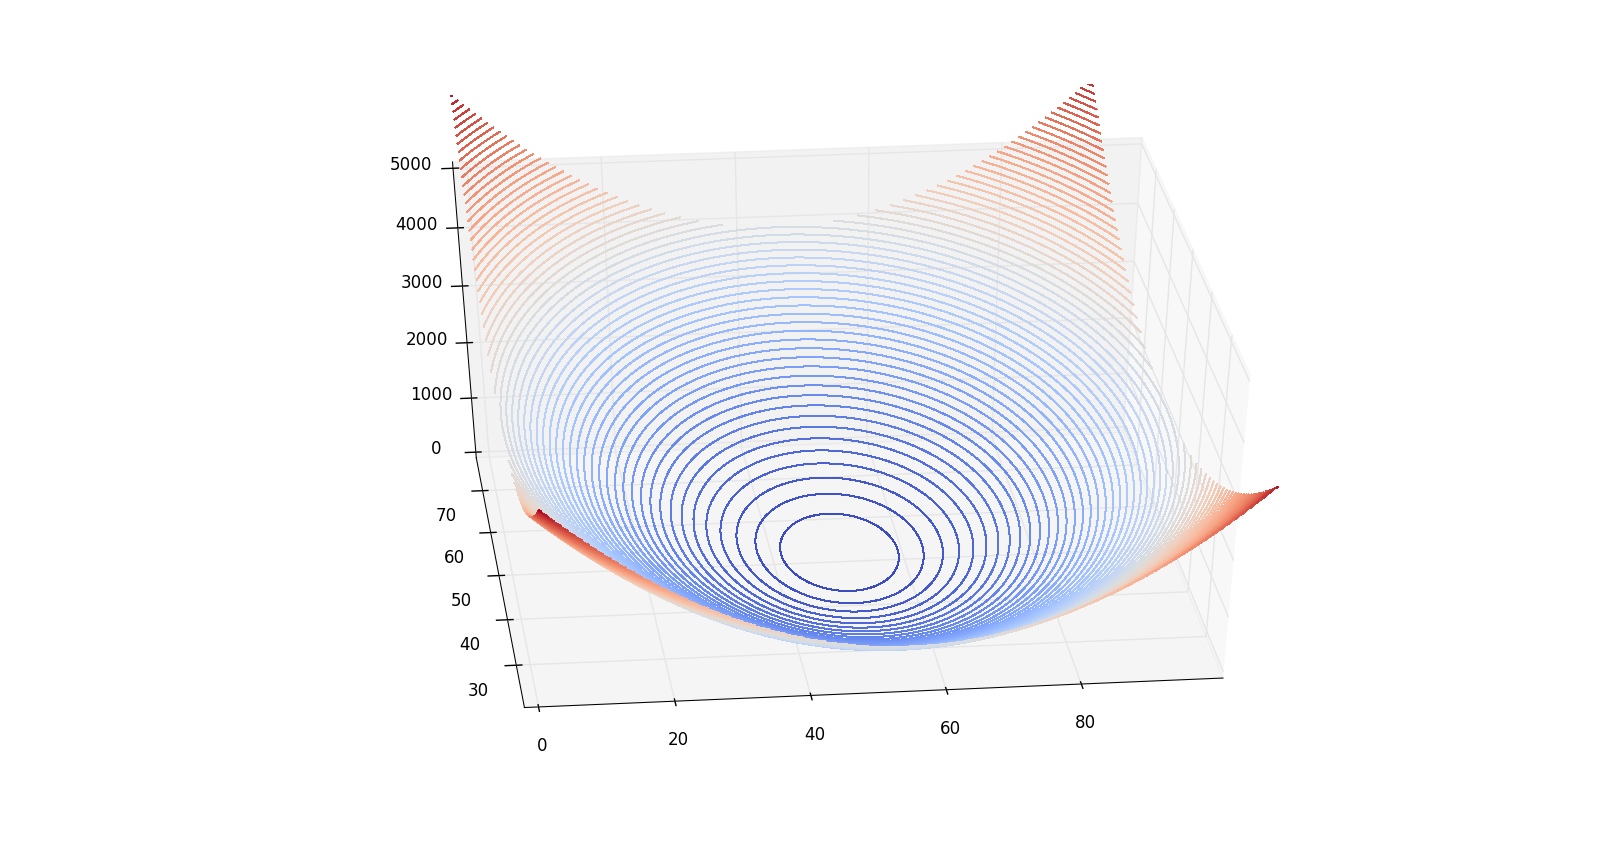
\includegraphics[height=.3\vsize]{fig/arriv1.png}
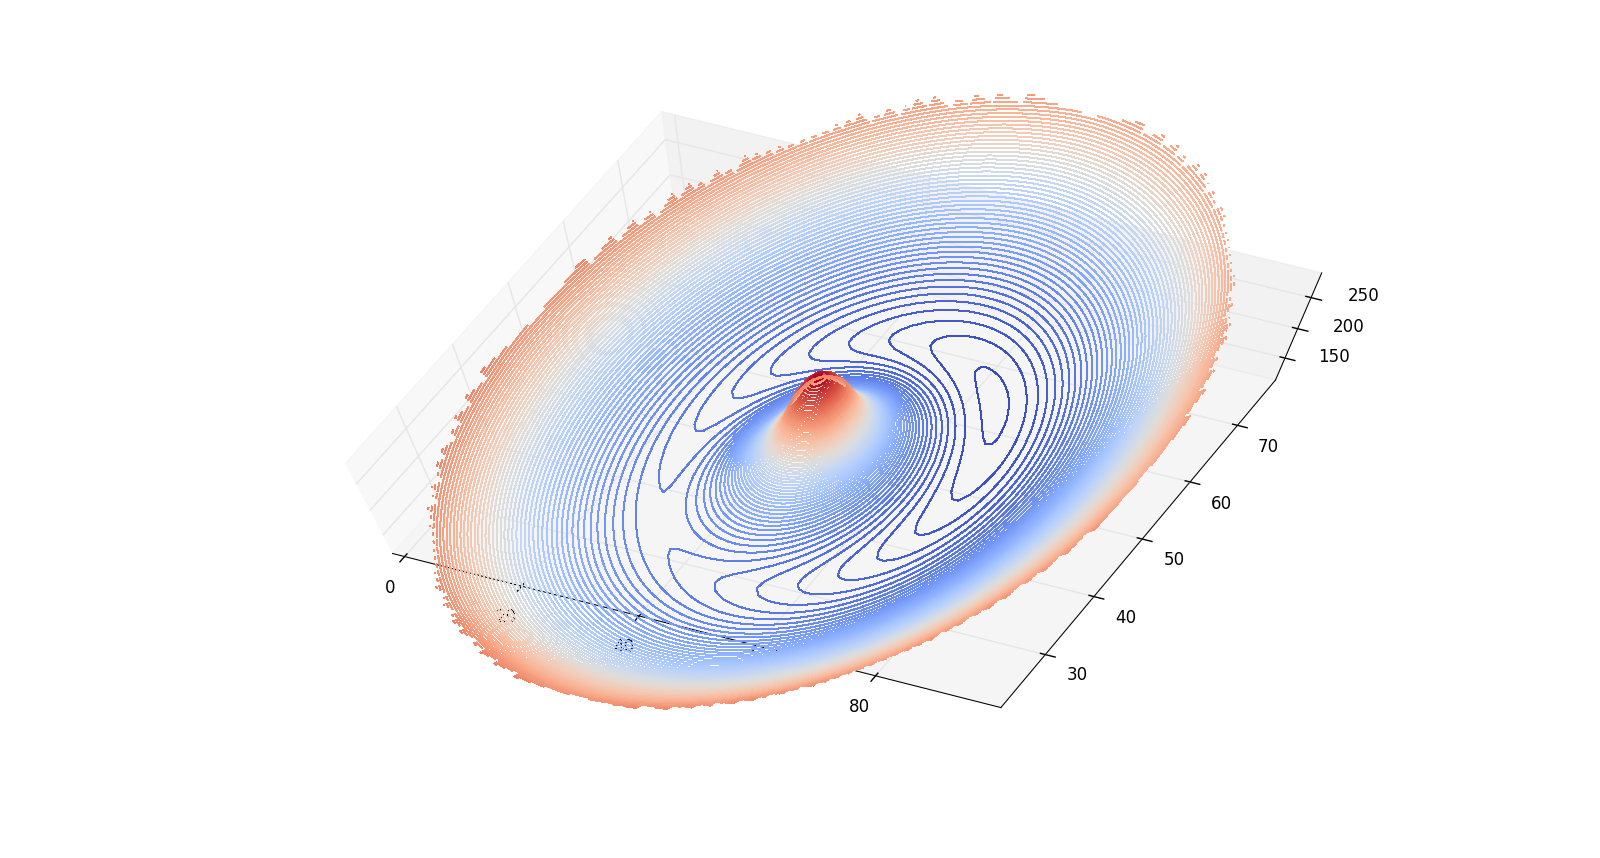
\includegraphics[height=.3\vsize]{fig/arriv2.png}
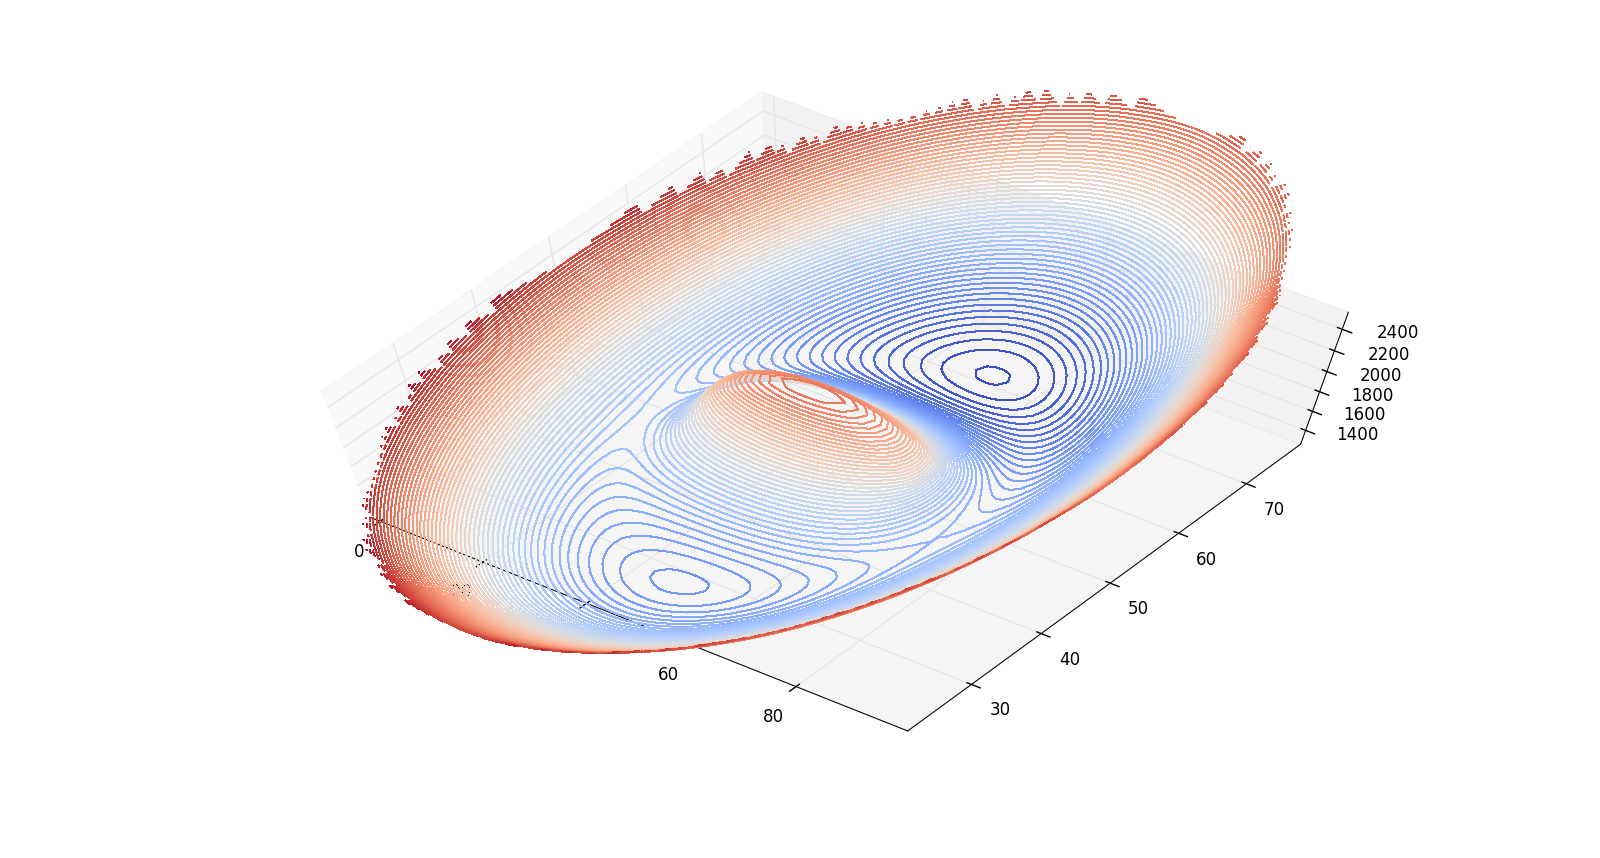
\includegraphics[height=.3\vsize]{fig/arriv3.png}
\caption{Arrival-time surfaces, with contour levels of equal arrival
  time.  The upper surface is with no lens.  The middle surface is
  when a circular lensing mass (offset from the source) is added; a
  maximum, a minimum and a saddle point can be seen.  The last surface
  is the result of an elongated lensing mass; a maximum, two minima
  and two saddle points can be seen.
}
\label{fig:arriv}
\end{figure}

Consider a gravitational lens.  As in most astrophysical lensing, this
lens is `thin' along the line of sight, and effectively lies on a
plane.  Let $x,y$ be coordinates on this plane.  These coordinates
measure ordinary physical lengths (metres, etc) on the lens plane.
Let there be a point source of light at $x=0,y=0$ but far behind the
lens plane.  Now imagine a light ray coming from the source to the
lens plane $(x,y)$ and then changing its path to reach the observer.
The observer would see the source apparently behind $(x,y)$ on the
lens.  If this happened, the light ray would have taken a longer path
than having come directly to the observer.  The geometrical path
difference would be $\propto x^2 + y^2$ for small angles.  Let us
define
\begin{equation} \label{eq:Ageom}
A_{\rm geom}(x,y) = \half(x^2 + y^2) \,.
\end{equation}
As written, this looks is an area.  But we can also think of it as a
time delay introduced by the light ray bending --- with an unwritten
constant factor.  That factor is basically the lens distance times the
speed of light; the precise expression has to take the expansion of
the Universe into account, and is given in the Appendix.  The top part
of \figref{arriv} shows what $A_{\rm geom}$ looks like: it is
just a paraboloid.  The minimum of the surface is at the source, and
that is where, according to Fermat's principle, the image will be.
The rest of the arrival-time surface is just an imaginary surface.

The geometrical time delay \eqref{eq:Ageom} is not the only one.  The
warping of space by a gravitational field introduces a further time
delay $A_{\rm grav}$.  The arrival time of the light ray, compared to
what it would have been with no lensing, is
\begin{equation} \label{eq:Aarriv}
\hbox{arrival time} = A_{\rm geom} + A_{\rm grav} \,.
\end{equation}
We can also express $A_{\rm grav}$ as an area, with the same implicit
constant factor that makes it a time.  The expression, however, is
more complicated.  We first introduce the notation $\nabla^2 f(x,y)$
to denote
\begin{equation}
 \frac{ f(x+\Delta x, y) + f(x-\Delta x, y) +
        f(x, y+\Delta y) + f(x, y-\Delta y) - 4 f(x,y) }
      {\Delta x \; \Delta y}
\end{equation}
in the limit of $\Delta x,\Delta y$ small.  Then we write the
projected mass density of the lens, which would be in $\rm
kg\,m^{-2}$, in special units (given in the Appendix) such that the
surface density becomes a dimensional field $\kappa(x,y)$.  Then
\begin{equation} \label{eq:Poisson}
\nabla^2 A_{\rm grav}(x,y) = -2\kappa(x,y) \,.
\end{equation}
Note that $A_{\rm grav}(x,y)$ is not given explicitly in terms of
$\kappa(x,y)$, but as a differential equation that must be solved.
Equations of the type \eqref{eq:Poisson} are, however, well known (as
Poisson equations in two dimensions), and there are techniques for
solving them.  Incidentally, $\kappa$ has a second meaning, as well as
being a dimensionless form of the the projected density: it also
measures how a bundle of light rays is brought together by
gravitational lensing, and is called the {\em convergence}.

What is the effect of mass on the arrival-time surface?  If the mass
distribution $\kappa(x,y)$ is circular, $A_{\rm grav}(x,y)$ will have
a peak at the centre of that circle.  But if the mass is not precisely
in front of the mass, the arrival-time surface will not be circular
any more.  The result is illustrated in the middle part of
\figref{arriv}.  In addition to the maximum, there is now a
minimum and a saddle point.  According to Fermat's principle, images
appear at maxima and saddle points as well as minima.  If the mass
distribution is non-circular, more images can appear.  The lower
example in \figref{arriv} shows the arrival-time surface due
to an elongated mass.  There is still a maximum, part of an elongated
hill, and around it there are two minima and two saddle points.

So far we have considered a single point source.  What if there is an
extended source?  To understand this, let us consider what happens if
we move the original point source slightly, or equivalently, keep the
original point source behind $x=0,y=0$ and move the lens slightly.
The contours of constant arrival time will, naturally, move slightly,
and so will the images.  The movement of the contours will be most
noticeable where the contours are far apart, that is, where the
arrival-time surface is nearly flat.  As is evident from
\figref{arriv}, this is the region where the minima and saddle
points lie, or near the images.  In this region, points on the source
that are close together produce images that are comparatively far
apart.  In other words, the image is highly magnified.  In summary,
lower curvature in the arrival-time surface for a point source implied
larger magnification of an extended source.  Conversely, where the
arrival-time surface is strongly curved, the image will be
demagnified.  We see from \figref{arriv} that the arrival-time
surface tends to be highly curved near the maximum.  Hence maxima tend
to be demagnified.  In practice, maxima of the arrival time are nearly
always too faint to see.  The minima and saddle points dominate.

In the lensed examples in \figref{arriv}, the maximum in each
case is evident, but how can we distinguish the minima from the saddle
points?  The key is to examine the contours of equal arrival time.
Contour curves loop around a minimum or a maximum, but near a saddle
point, the contours do not loop around, instead they approach and then
pull away.  The contour curve precisely level with a saddle point
forms an X at the saddle point.  In \figref{arriv}, one such X
is evident.  In other cases the X contour passing through the saddle
point is not itself plotted, but we can tell the other contours where
the X would be.  These self-crossing contours will play a special role
in the following.

